
\section{System Implementation}
Centered around the PC object model, TCAP compiler and PC pipeline execution, we've built a distributed system to manage large scale PC objects and support user queries and analytics workloads, as illustrated in Fig.~\ref{fig:arch}.

\begin{figure}
\centering
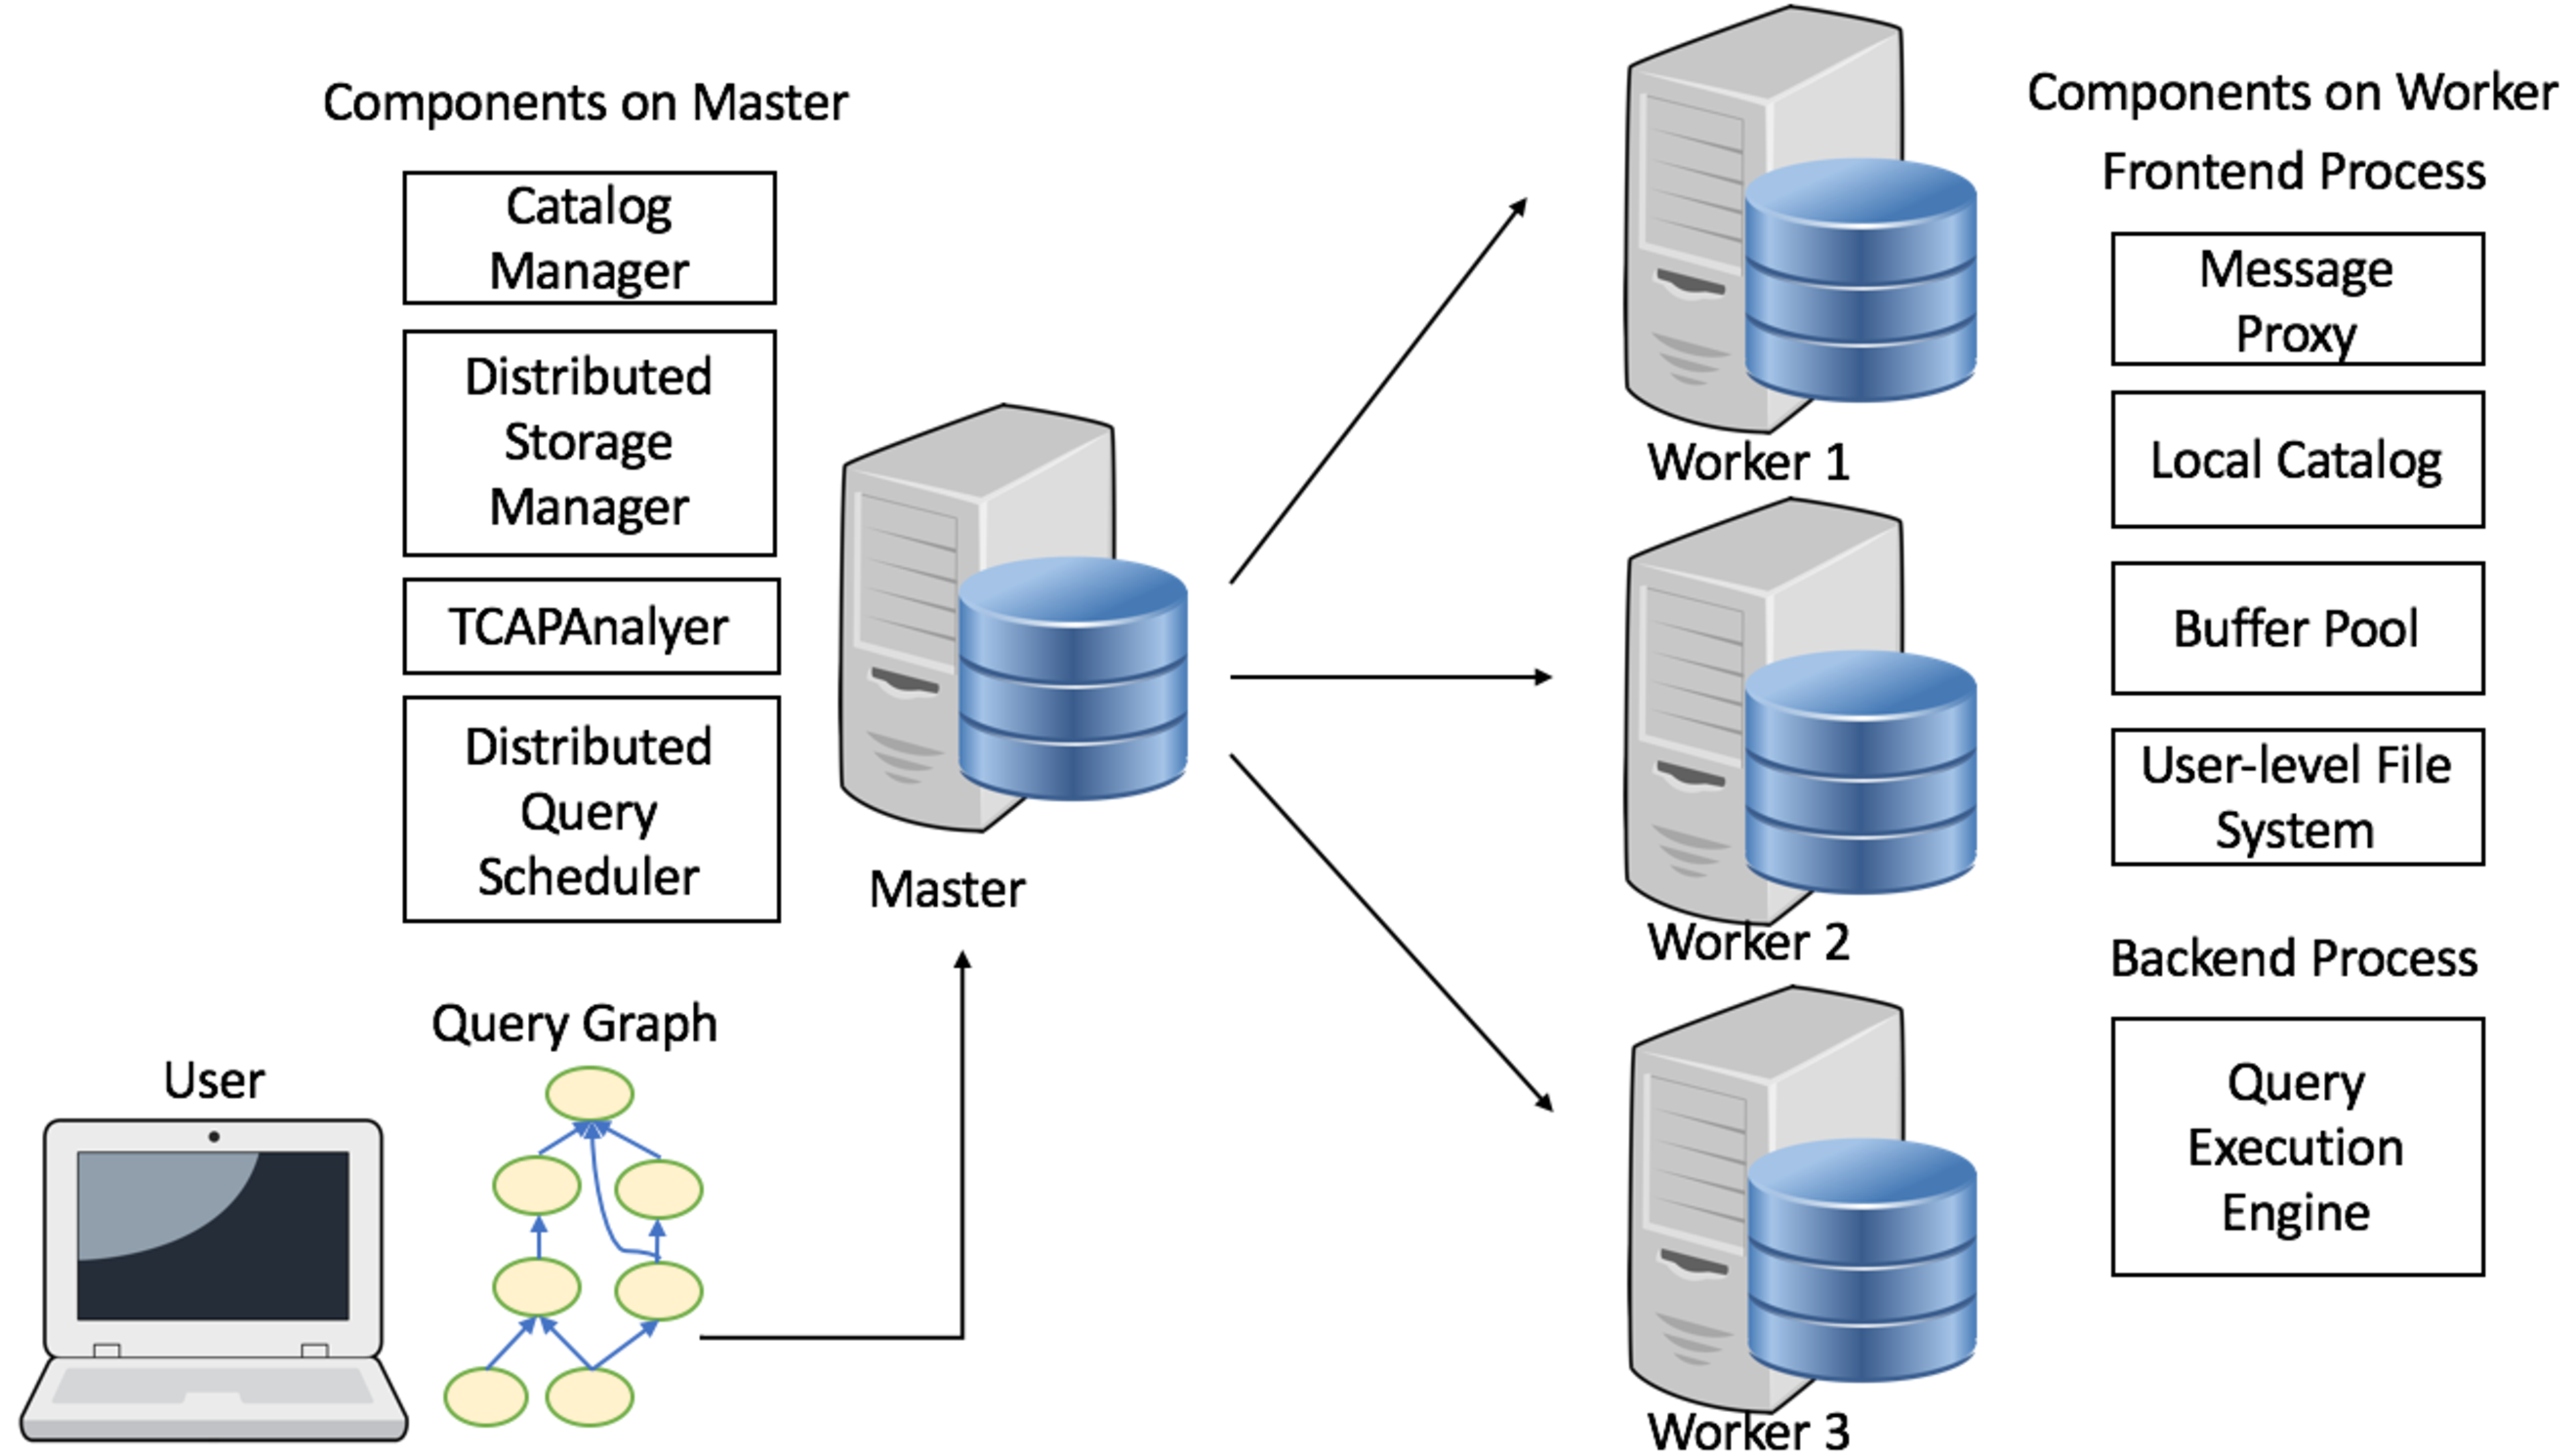
\includegraphics[width=0.75\textwidth]{arch.pdf}
  \caption{\label{fig:arch} PC distributed runtime.}
\end{figure}

The Master server contains four components: 

\begin{enumerate}
\item \emph{Catalog Manager}, serving system meta-data as well as dynamically-loaded code for performing computation over PC \texttt{Object}s;
\item \emph{Distributed Storage Manager}, a centralized server functionality to manage storage subsystem in each worker server to perform Create, Read, Update, Delete operations over datasets of PC \texttt{Object}s across a distributed cluster.
\item \emph{TCAP Optimizer},  responsible for optimizing programs that have been compiled into PC's domain-specific TCAP langague.
\item \emph{Distributed Query Scheduler}, responsible for accepting optimized TCAP computations, dynamically schedule job stages from TCAP, and executing the compiled TCAP code on the cluster for each job stage.
\end{enumerate}

Each worker machine in a PC cluster runs two processes: a frontend process and a backend process.
Dual processes are used because PC executes potentailly unsafe native user code.  By definition, user code is run only in the backend process---if            
user code happens to crash the backed process, it can be restarted by the front end.

The frontend process runs following components:

\begin{enumerate}
\item \emph{Local Catalog}, storing local meta data and dynamically-loaded code dispatched to this worker;
\item \emph{Storage Server}, a local storage server that manages a shared-memory buffer pool used for buffering and caching datasets and a user-level file system used to store persist datasets or data spills. The buffer pool shared memory is created via mmap system call, so data stored in it can be read by backend process (which is forked from the frontend process) through zero-copy access. The local storage server manages a number of datasets. Each dataset consists of one or more pages (with default size being 256 mega bytes), which can be cached in buffer pool and/or spill to the user-level file system.
\item \emph{Message Proxy},  responsible for communicating with backend process to bridge the Master Server, local catalog, local storage server and the backend process.

\end{enumerate}

The backend process consists of a query execution engine that executes various types of computation, such as selection, multiselection, aggregation, broadcast join, hashPartitioned join, topK and so on. Here we describe the execution of aggregation and hash partition join as two examples.


\subsection{Query Processing Examples}
\subsubsection{Aggregation Example}
As shown in Fig.~\ref{fig:aggregation},  PC aggregation implementation provides high performance service based on (i) the object model that avoids serialization and deserialization overhead when shuffling data; (ii) decomposing the complex multi-producer/multi-consumer processing into a set of multi-threading stages connected by zero-copy and low-synchronization pointer queues to avoid materializing intermediate data and avoid overcommiting resources when demand exeeds service capacity; (iii) employment of dynamic control to automatically tune runtime parameters (e.g. number of threads and buffer size for each stage) to improve resource utilization. 

\begin{figure}
\centering
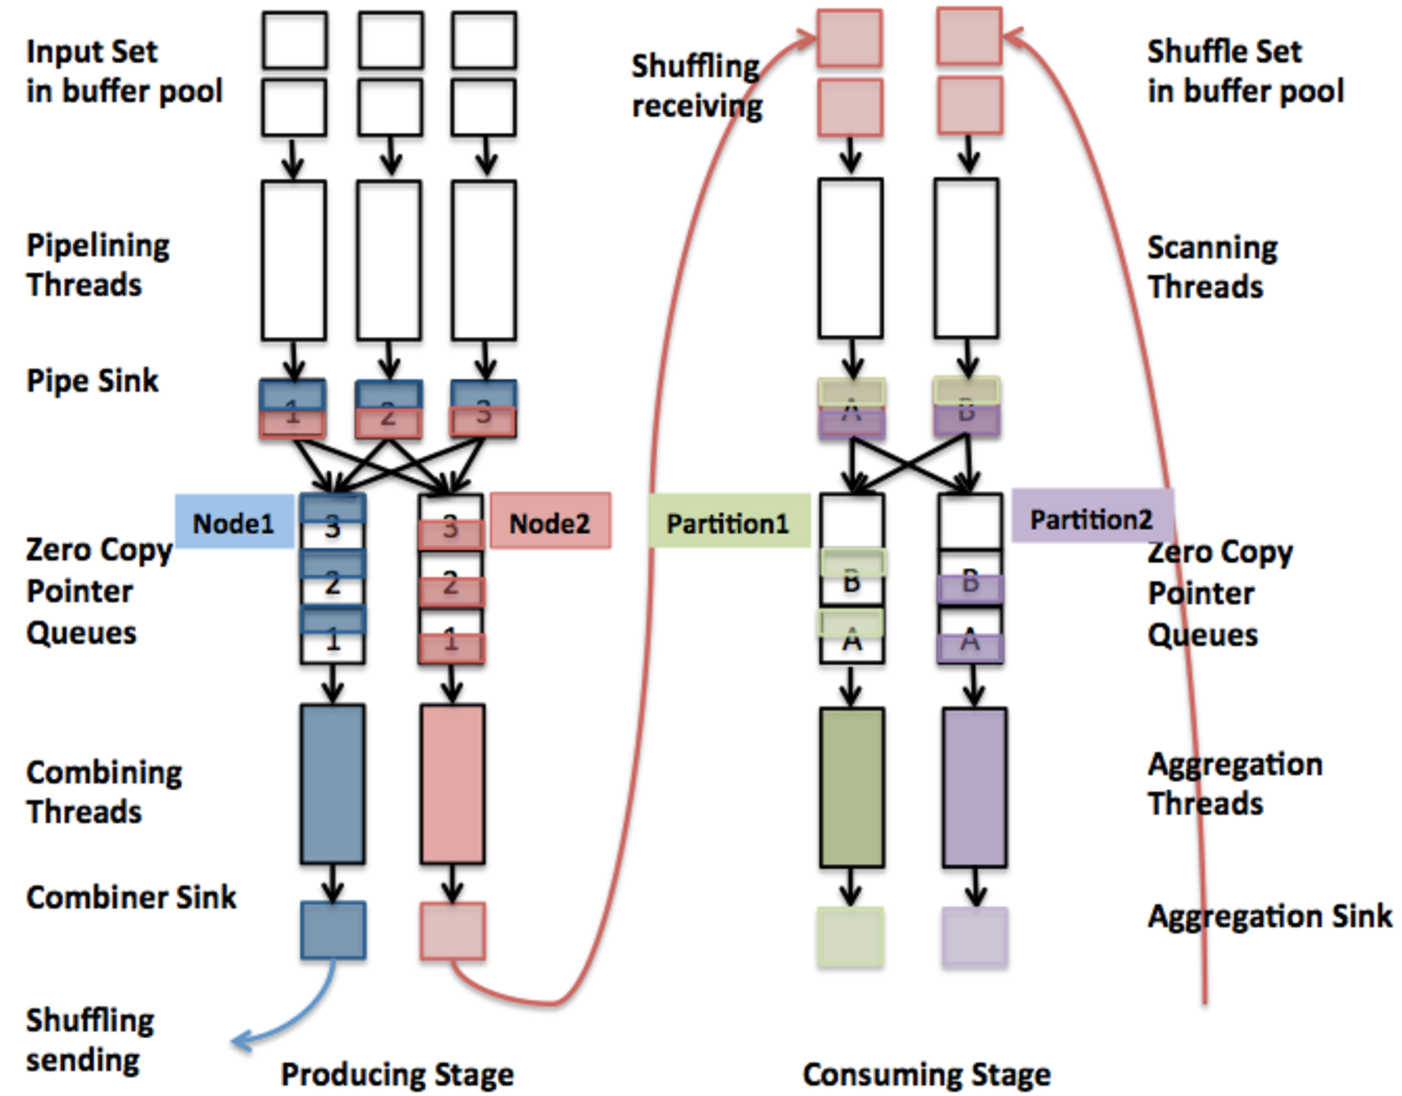
\includegraphics[width=0.75\textwidth]{aggregation.pdf}
  \caption{\label{fig:aggregation} Aggregation Implementation Illustration.}
\end{figure}

As illustrated in Fig.~\ref{fig:aggregation}, the distributed query scheduler server will schedule an Aggregation computation into two consecutive JobStages. The first JobStage do the pre-aggregation and shuffle pre-aggregation results to each other worker, so that each worker have all the data for a number of partitions. The second JobStage completes the aggregation for each partition. The details are described as following.

\vspace{5pt}
{\bf 1. Producing Stage.} This stage consists of $N$ pipelining threads to scan and process pages in the input set. An input page has a container Vector$<$Object$>$ or Map$<$Object$>$ to hold input objects to process. Each pipeline thread will invoke makeObjectAllocatorBlock() to allocate a temporary page to write intermediate data and output key-value pairs. Each such temporary page is allocated in heap and has a handle to container Vector$<$Map $<$Object, Object$>$$>$ as the pipe sink, where each Map Object corresponds to a hash partition. 

When pipeline threads start running, each pipeline thread iteratively generates batches of Objects from the container in the input page. A batch, called as a tuple set, typically consists of hundereds of Objects to amortize function call overhead and also fit intermediate data to cache size to avoid OS cache miss and page faults overhead. For each tuple set, the pipeline thread applies the a series of lambda functions that are compiled from TCAP to each batch. In the end, for each tuple in the tuple set the pipeline transforms it into a key-value pair. Then the key in the pair will be hashed to match the hash partition that the key-value pair belongs to and then the pair will be inserted to the Map$<$Object, Object$>$ in the container that corresponds to the hash partition.

In the same time, $K$ combining threads are running in local to pre-aggregate key-value pairs for hash partitions allocated for a specific cluster node. 

To efficiently pass the pipe sink pages to combining threads with minimum memory copy and synchronization overhead, we provide a zero-copy pointer queue structure to connect pipelining threads to combining threads. Once a pipe sink page becomes full, we get the pointer to that page, and append the pointer to each combining thread's pointer queue ( and allocate a new temporary page for pipe sink ). Then each combining thread can read the container in the same page in parallel, but will only select from the container a subset of hash partitions that it is responsible for to process. We maintain a reference count for each page, before appending a Record pointer to the all the queues, we increment the reference count to be the total number of queues. Later for each dequeue operation, the reference count will be decremented. The page data will only be freed from heap when reference count reduces to zero. 

Each combining thread writes pre-aggregated key-value pairs of its responsible partitions, also in the form of Vector$<$Map$<$Object, Object$>$$>$, to a thread-local combiner page that can have arbitrary size (automatically tuned to use as much memory as possible). 

Once a combiner page becomes full, the container in the page is directly sent to the corresponding cluster node for final aggregation and a new combiner page will be allocated. Each node stores received container into a shuffle set that is created in buffer pool and will be processed in the consuming stage. Because all objects are inherited from Object or be simple C++ type, there is no need to serialize/deserialize data for shuffling. Compression can be enabled to reduce shuffle data size through configuration.
 
\vspace{5pt}
{\bf 2. Consuming Stage.} This stage consists of $N$ scanning threads and $M$ aggregation threads. Each aggregation thread is responsible for one hash partition,  so $M$ is the total number of partitions on each node.

Similar with combining in the Producing stage, each aggregation thread has a zero-copy pointer queue that connects to all scanning threads.

Scanning threads retrieve different subsets of pages from the shuffle set, and append the pointer to each shuffle page to each aggregation thread's incoming queue, so that all aggregation thread can find and process its own partition in all shuffle pages in parallel. For each shuffle page, an aggregation thread first gets the Handle to the Vector$<$Map$<$Object, Object$>$$>$ container, and then gets the Handle to the Map partition in the Vector container that this aggregation thread is responsible for. Each aggregation thread allocates a large enough page in the heap to serve as thread-local allocation block, and creates a Map$<$Object, Object$>$ container in the allocation block to write aggregation results to serve as aggregation sink. So each Key Value pair in the source maps extracted from shuffle pages is inserted and aggregated to the aggregation sink. 

All aggregation sinks form a special set, called partitioned hash set. The lifetime of input set, shuffle set and hash set are managed automatically by the distributed query scheduler component.


\vspace{5pt}

On each node, all parameters like number of hash partitions $M$, number of pipelining threads $N$, number of combining threads for each remote node $K$, combiner page size, and aggregation page size are all automatically determined at run-time to maximize memory utilization, network utilization and CPU utilization. For example, $M$ and $N$ are tuned to be proportional (1.5 times by default) to CPU core number on each node, $K$ is tuned as a trade-off between context switch overhead and amount of data that needs to be shuffled, so we reduce $K$ when there are a lot of remote nodes to shuffle data to reduce context swith overhead and we increase $K$ when the data to shuffle increases to be able to transfer data to consumer in time. Combiner page size and aggregation page size are all tuned to be the total free memory multiplied by a pre-configured ratio (0.8 by default) to maximize memory utilization. 

\subsubsection{Hash Partition Join Example}

The distributed query scheduler server schedules a $K$-way hash partition join into $2K$ job stages. Each of the first $K-1$ input needs two job stages to repartition data and build (and co-locate) hash table for each partition respectively. Then the last input requires one job stage to repartition data and  another job stage, which is the final stage, to join $K$ inputs for each partition. Now we describe the data repartition stage, hash table building stage, and the final hash partition join stage respectively.

\vspace{5pt}
{\bf 1. Data Repartition Job Stage.} This job stage is similar with the Producing stage in aggregation, but it uses a different type of container to write to the pipe sink. 

$N$ pipelining threads work together to read tuple sets from a source set, applies a series of lambda functions compiled from TCAP to each tuple set in a vectorized processing style. In the end, each tuple in the tuple set will be transformed into a key-tuple pair and written to a Vector$<$Map$<$Object, Vector$<$Object$>$$>$$>$ container in the pipe sink page.  Each Map is corresponding to a hash partition. 

Once there is no more free memory in the pipe sink page, instead of send each Map to its destination node, we append the pointer of that page to the queue of each combining thread, just like the Producing stage in aggregation. Each of $K$ combining threads correspond to a node in the cluster, so it picks up the Map objects that are partitioned to that node, and writes them to a new container in the thread's local combiner page that is dedicated for that node.

Once a combiner page is full, it will be compressed, sent to the destination node, decompressed and directly put as a page to a shuffle set in the buffer pool, and no serialization and deserialization is required in this shuffling process.

\vspace{5pt}
{\bf 2. Hash Table Building Job Stage.} This job stage is similar with the Consuming stage in aggregation, except  that it uses different types of containers as sources and sinks. 

$N$ scanning threads and $M$ Map merging threads are running. Each Map merging thread is responsible for one hash partition,  so $M$ is the total number of partitions on each node.

Scanning threads retrieve different subsets of pages from the shuffle set, and append the pointer to each shuffle page to each Map merging thread's incoming queue, so that all Map merging thread can find and process its own partition in all shuffle pages in parallel. For each shuffle page, a Map merging thread first gets the Handle to the Vector$<$Map$<$Object, Vector$<$Object$>$$>$$>$ container, and then gets the Handle to the Map partition in the Vector container that this Map merging thread is responsible for, which is called a source Map. Each Map merging thread allocates a large enough page in the heap to serve as thread-local allocation block, and creates a Map$<$Object, Vector$<$Object$>$$>$ container in the allocation block, as sink Map. Then the Map merging thread iterates the source Map, and put each key-tuple pair iterated to the sink Map. Once a source Map is fully merged, the Map merging thread will fetch a new source Map from the next shuffle page, and repeats the process until all Maps are merged for this partition.



\vspace{5pt}
{\bf 3. Hash Join Job Stage.} Once each of the first $K-1$ input has been transformed to a partitioned hash table, and the $K$-th input has been repartitioned and stored as shuffle sets in each node, the same partition for all inputs should be co-located in the same machine. 

Then this final job stage is run to complete the join operation. It allocates one pipeline thread for each partition on each machine. The source of the pipeline thread is the shuffle set caching the partitioned data of the $K$-th input, and the sink can be an output dataset that is buffer cached in buffer pool and persisted to the user-level file, or can be an intermediate dataset that just needs to be cached in buffer pool and does not need to be persisted to disk. 

Each pipeline thread reads the tuple sets from the source set, probes the hash tables of other $K-1$ inputs, and write joined results to the sink set.

\subsection{Dynamic Query Scheduling}
Now we briefly describe the implementation of dynamic scheduling of job stages. 

A TCAP compiler compiles the TCAP automatically coded from user query graph into a query plan that is a graph connecting TCAP instructions with native code generated for executing each instruction. 

Then the TCAP analyzer will search the query graph to look for the best job stage to execute, based on a cost model that considers size of source sets, size of sink set and data locality. The goal is to minimize generated intermediate data size,  and in the same time to execute all computations that are related with one dataset as close as possible to improve memory locality and avoid unnecessary data eviction from memory.

Once the optimal job stage is identified, the distributed query scheduler will allocate datasets through the distributed storage manager, schedule the stage to run across the cluster, collect the statistics such as the size of result datasets, and remove unused datasets. Then based on the updated statistics, a new job stage will be identified as the optimal one and get scheduled until the query plan has been fully executed.